\chapter{Marchés et régulations}
\section{La concurrence en Europe}
La politque globale de l'Europe est de mettre en place la concurrence partout ou cela est possible. En effet, la mise en concurrence des entreprises permet de faire baisser les prix pour les consommateurs et donc de réduire l'inflation. Cependant, la concurrence parfaite n'existe pas. Il faut donc que l'Europe puisse appliquer plusieurs politiques pour \textbf{réguler} ces phénomènes. Il y a une surveillance des insitutions visant à réduire les "monopoles naturels", à instaurer des politiques environnementales... \newpage

\subsection{Loi de l'offre et la demande}
\begin{center}
    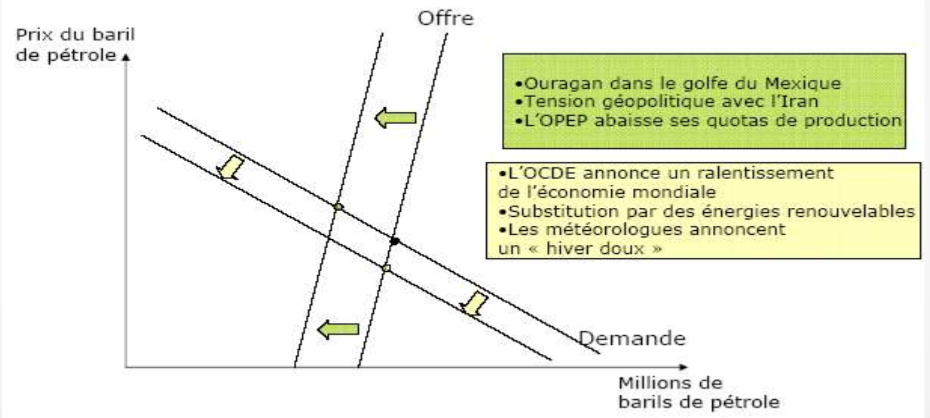
\includegraphics[scale=0.7]{Pics/Offre_et_demande.png}    
\end{center}
$(Offre \searrow + demande = cste) \implies Prix \nearrow$ \newline
$(Offre \nearrow + demande = cste) \implies Prix \searrow$ \newline
$(Demande \searrow + offre = cste) \implies Prix \searrow$ \newline
$(Demande \nearrow + offre = cste) \implies Prix \nearrow$
\subsection{Courbe de l'offre en situation de concurrence}
\begin{center}
    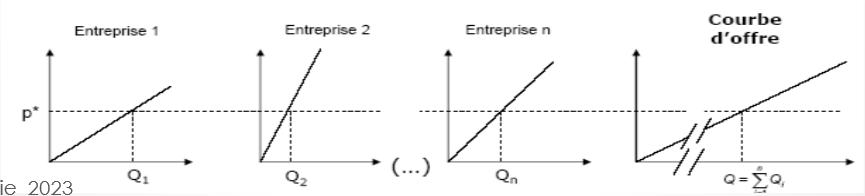
\includegraphics[scale=0.8]{Pics/Courbe_de_l_offre.png}
\end{center}
\newpage
\subsection{Elasticité-prix $\epsilon$ de la demande}
\begin{center}
    \fbox{\huge{$\epsilon = \frac{\frac{dQ}{Q}}{\frac{dp}{p}} = \frac{dQ}{dp}\frac{p}{Q}$}}   
\end{center}
Mesure de la variation de la quantité d'un produit par rapport à la variation de son prix
p : prix du produit \newline
q : quantité du produit
\begin{itemize}
    \item $\epsilon = 0 $ : inélasticité
    \item $\epsilon \in [-1;0[$ : faiblement élastique
    \item $\epsilon \in ]-\infty;-1]$ : élastique
\end{itemize}
\subsection{Elasticité à court et à long terme}
Il faut un certain  temps avant que la quantité d'un produit se stabilise face à une variation de prix
\begin{center}
    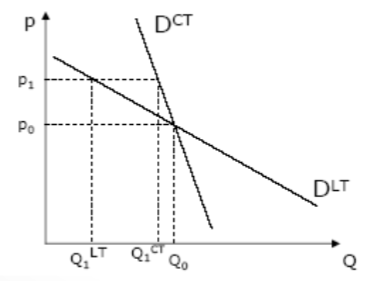
\includegraphics[scale = 1]{Pics/elasticite_court_et_long_terme.png}
\end{center}
\newpage
\subsection{Elasticité des prix croisés de la demande}
C'est la mesure de la déportation d'un produit A vers un produit B lorsque le prix de A augmente.
\begin{center}
    \huge{\fbox{$\epsilon_{i,j} = \frac{\frac{\partial Q_{i}}{Q_{i}}}{\frac{\partial p_{j}}{p_{j}}}=\frac{\partial Q_{i}}{\partial p_{j}}\frac{p_{j}}{Q_{j}}$}}
\end{center}
\begin{itemize}
    \item Si $\epsilon_{i,j} > 0 $: les biens sont substituables
    \item si $\epsilon_{i,j} < 0 $: les biens sont complémentaires
\end{itemize}
\begin{center}
    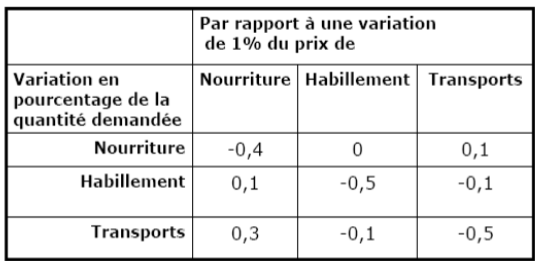
\includegraphics[scale=0.8]{Pics/elasticite_prix_croises.png}
\end{center}
\subsection{Elasticité revenu de la demande}
C'est la mesure de l'évolution du revenu réel du consommateur et de l'évolution de la quantité de produit.
\begin{center}
    \huge{\fbox{$\epsilon_{R} = \frac{\frac{dQ}{Q}}{\frac{dp}{p}}=\frac{dQ}{dp}\frac{p}{Q}$}}
\end{center}
\begin{itemize}
    \item Si $\epsilon_{R} > 1 $: le bien est dit \textbf{de luxe}
    \item si $\epsilon_{R} < 0 $: les biens est dit \textbf{inférieur}
\end{itemize}
\newpage
\section{La technologie de l'entreprise}
Conditions de production de l'entreprise :
\begin{itemize}
\item facteurs de production : 
    \begin{itemize}
        \item $K$ : capital\footnote{Ex : nombre d'heures de fonctionnenment des machines}
        \item $L$ : travail \footnote{Ex : nombre d'heures de travail}
        \item w : taux de salaire horraire
        \item r : coût horraire du capital
    \end{itemize}
\item Fonction de production
    \begin{itemize}
        \item $Q = f(K,L)$
    \end{itemize}
\item Fonction coût de l'entreprise
    \begin{itemize}
        \item $CF$ : coût fixe
        \item $CV(Q)$ : coût variable
    \end{itemize}
\end{itemize}
Fonction de coût total :
\begin{center}
    \Large{\fbox{$CT(Q) = CF + CV(Q)$}}
\end{center}
Fonction de coût moyen :
\begin{center}
    \Large{\fbox{$CM(Q) = \frac{CT(Q)}{Q} = \frac{CF}{Q} + \frac{CV(Q)}{Q}$}}
\end{center}
Fonction de coût marginal :
\begin{center}
    \Large{\fbox{$Cm(Q) = \frac{dCT(Q)}{dQ} = \frac{dCV(Q)}{dQ}$}}
\end{center}
\newpage
\section{Concurrence parfaite}
Comportement de la firme en situation de concurrence :
\begin{itemize}
    \item $\pi$ : profit de l'entreprise
\end{itemize}
Maximisation du profit de l'entreprise, en situation de \textbf{price taker}\footnote{L'entreprise est "preneuse de prix" : elle n'a pas le pouvoir d'influencer les prix sur le marché} : 
\begin{center}
    \Large{\fbox{$\max \pi (Q) = pQ - CT(Q)$}}
\end{center}
Condition de premier ordre :
\begin{center}
    \Large{\fbox{$\frac{d\pi(Q)}{dQ} = 0$}}
\end{center}
\begin{center}
    \Large{$\frac{d\pi(Q)}{dQ} = p - \frac{dCT(Q)}{dQ} = 0 \Longleftrightarrow p - C_{m}(Q) = 0$}
\end{center}
L'entreprise produit une quantité \textbf{à l'équilibre en situation de concurrence parfaite} $Q$ tq :
\begin{center}
    \Large{\fbox{$p=C_{m}(Q)$}}    
\end{center}


Comportement des entreprises sur un marché : plus il y a des opportunités dans un secteurs, plus les entreprises vont vouloir entrer dans ce secteur, ce qui a pour conséquences d'augmenter l'offre et donc de faire baisser les prix. \newline
Conditions de la concurrence parfaite:
\begin{center}
    \begin{itemize}
    \item Atomicité
    \item Biens homogènes
    \item libre entrée
    \item information parfaite
    \item Biens exclusifs
\end{itemize}
\end{center}
\newpage
\subsection{Dynamique de la concurrence parfaite}
Au bout d'un temps suffisament long, les profits $\pi$ des entreprises sont nuls et $p=CM=C_{m}$
\begin{center}
    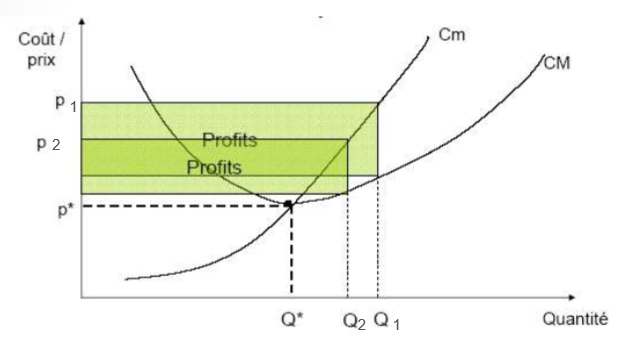
\includegraphics[scale=0.8]{Pics/dyn_concu_parfaite.png}
\end{center}
Rendements de la fonction de production : \newline
La fonction de production a 
\begin{itemize}
    \item Un rendement constant si :
    \begin{center}
        \Large{\fbox{$\lambda Q = f(\lambda K, \lambda L)$ avec $\lambda>1$}}
    \end{center}
    \item Un rendement décroissant si :
    \begin{center}
        \Large{\fbox{$\lambda Q < f(\lambda K, \lambda L)$}}
    \end{center}
        \item Un rendement croissant si :
    \begin{center}
        \Large{\fbox{$\lambda Q > f(\lambda K, \lambda L)$}}
    \end{center}
\end{itemize}
Fonction à rendement constant (fonction de Cobb-Douglas)
\begin{center}
    \Large{$Q = K^{\alpha}L^{\alpha}$}
\end{center}
\newpage
\subsection{Surplus du consommateur}
le surplus du consommateur est la mesure du taux de satisfaction client. C'est la différence entre le prix qu'il aurai payé pour le produit et le prix qu'il paye réellement.

avec :
\begin{itemize}
    \item $S$ : satisfaction
    \item $Q^{*}$ : quantité échangée
    \item $p^{*}$ : prix échangé
\end{itemize}
\begin{center}
    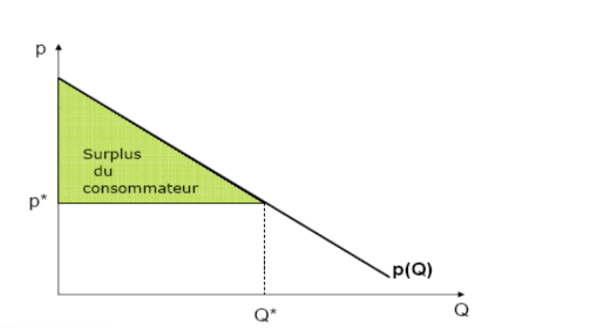
\includegraphics[scale=0.8]{Pics/surplus_consommateur.png}
\end{center}
\newpage
\section{Les défaillances du marché}
\subsection{Biens économiques}
Biens économiques : ils sont rivaux ou non, avedc un certain degré d'exclusivité
\begin{itemize}
    \item \textbf{Bien rival} : deux agents ne peuvent pas en bénéficier en même temps de ce bien \footnote{Bien rival = bien exclusif - ex : une voiture, tragédie des biens communs $\neq$ biens non-rivaux}
    \item \textbf{Bien exclusif} : bien que peut disposer l'agent que s'il paye le prix \footnote{ex : chaîne de télévision, logiciel, biens publics $\neq$ biens non-exclusifs}
\end{itemize}
Les biens et services de consommation privée traditionnelle sont les deux à la fois.
\subsection{Externalité}
C'est un effet subit par un agent économique au cours d'une action de consommation ou de production \footnote{Ces externalités sont trop ou pas assez produites, en fonciton de leurs types : il faut alors taxer et/ou subventionner certaines externalités pour les réguler.}
\begin{itemize}
    \item \textbf{Externalité positive} : effets de la R\&D, recherche publique sur la R\&d, recherche privée
    \item \textbf{Externalité négative} : effet de la pollution dûs aux rejets d'une usine
\end{itemize}
\begin{center}
    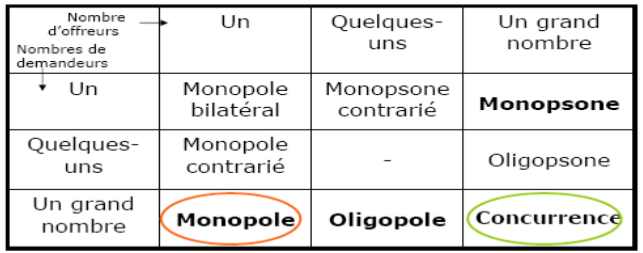
\includegraphics[scale=0.7]{Pics/defaillance_marche.png}
\end{center}
\newpage
\section{Le monopole}
\subsection{Comportement de l'entreprise}
Comportement de l'entreprise en situation de monopole
\begin{itemize}
    \item $\pi$ : profit de l'entreprise
    \item $Q(p)$ : fonction de demande
\end{itemize}
Maximisation du profit de l'entreprise, en situation de \textbf{price maker}\footnote{C'est l'entreprise qui fixe les prix}
\begin{center}
    \Large{\fbox{$max \pi(Q) = p(Q)Q - CT(Q)$}}
\end{center}
Condition de premier ordre :
\begin{center}
    \Large{\fbox{$\frac{d\pi(Q)}{dQ}=0$}}
\end{center}
\begin{center}
    \Large{$\frac{d\pi(Q)}{dQ} = \textcolor{BrickRed}{\frac{dp(Q)}{dQ}Q + p(Q)} - \textcolor{green}{\frac{dCT(Q)}{dQ}} = 0$}
\end{center}
\begin{itemize}
    \item\fbox{\textcolor{BrickRed}{$\frac{dp(Q)}{dQ}Q + p(Q) = R_{m}(Q)$}} la recette marginale \newline
    \item \textcolor{green}{$\frac{dCT(Q)}{dQ} = C_{m}(Q)$} le coût marginal \newline
    \item $\epsilon = \frac{dQ}{dp}\frac{p}{Q}$ (pour rappel)
\end{itemize}
Donc
\begin{center}
    $R_{m}(Q) = \frac{dp(Q)}{dQ}Q + p(Q) = \frac{1}{\epsilon}p(Q) + p(Q)$
\end{center}
on a alors \textbf{a l'équilibre d'une situation de monopole :}
\begin{center}
    \Large{\fbox{$R_{m}(Q) = C_{m}(Q)$}} \newline
    \textcolor{White}{.} \newline
    \Large{\fbox{$p(Q)(1+\frac{1}{\epsilon}) = C_{m}(Q)$}}
\end{center}
\newpage
Prix de monopole :
\begin{center}
    \LARGE{\fbox{$p(Q) = \frac{C_{m}(Q)}{1+\frac{1}{\epsilon}}$}}
\end{center}
En considérant la demande élastique (marché sur une échelle de temps longue soit $\epsilon \in ]-\infty;-1]$) :
\begin{center}
    \Large{$p^{M} = \frac{C_{m}(Q)}{1+\frac{1}{\epsilon}} > C_{m}(Q) = p^{C}$}
\end{center}
\begin{itemize}
    \item $p^{M}$ : prix du marché en situation de monopole
    \item $p^{C}$ : prix du marché en situation de concurrence
\end{itemize}
Marge :
\begin{center}
    \Large{\fbox{$M = \frac{p^{M}}{C_{m}}$}}
\end{center}
Taux de marge :
\begin{center}
    \Large{\fbox{$T_{m} = \frac{p^{M} - C_{m}}{C_{m}}$}}
\end{center}
\subsection{L'inefficience du monopole}
\begin{center}
    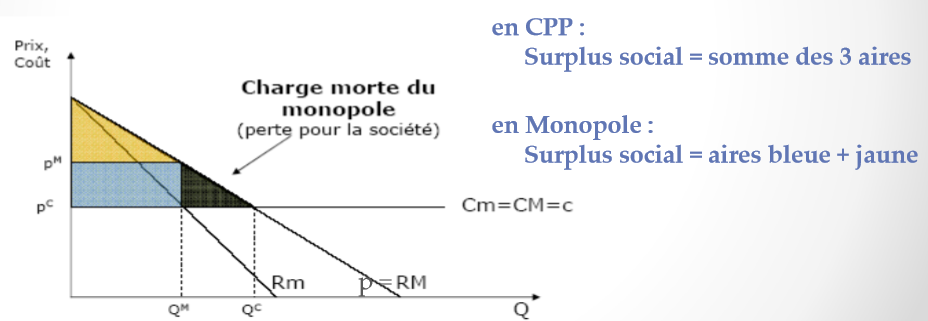
\includegraphics[scale=0.7]{Pics/Inefficience_monopole.png}
\end{center}
\newpage
\section{Les interractions stratégiques (ententes)}
Les situations de concurrence et de monopole sont deux structures de marché extrêmes et ne reflètent pas la réalité. En efft, il existe des phénomènes d'interdépendance et de startégies d'entreprises qui mènent à des ententes entres entreprises. \newline

\textbf{\textcolor{BrickRed}{Oligopole}} : nombre limité de grandes entreprises réalisant une part très importante de la production du secteur.
\newline
\begin{itemize}
    \item \textbf{Duopole de Cournot} : la quantité produite est la variable explicative de ces phénomènes \newline
    \item \textbf{Duopole de Bertrand} privilégie le prix \newline
    \item \textbf{Duopole de Stackelberg} : rôle des entreprises asymétrique (leader/follower)
\end{itemize}
\newpage
\subsection{Duopole de Cournot}
Soient deux entreprises qui produisent une quantité $q_{1}$ et $q_{2}$ de produits. Les coûts totaux sont $c_{1}q_{1}$ et $c_{2}q_{2}$. \newline
\begin{itemize}
    \item Quantité totale produite : \newline
    \textcolor{White}{.}
        \begin{center}
            \Large{\fbox{$Q = q_{1} + q_{2}$}}
        \end{center}
    \textcolor{White}{.}
    \item Fonction de demande inverse : \newline
    \textcolor{White}{.}
    \begin{center}
        \Large{\fbox{$p(Q) = p(q_{1} + q_{2}) = A - (q_{1} + q_{2})$}}
    \end{center}
    \textcolor{White}{.}
    \item Maximisation du profit de l'entreprise 1 et 2 : \newline
    \textcolor{White}{.}
        \begin{center}
            \begin{itemize}
                \Large{\fbox{$max  \pi(q_{1},q_{2}) = p(q_{1},q_{2})q_{1} - c_{1}(q_{1})$}} \newline
                \Large{\fbox{$max  \pi(q_{1},q_{2}) = p(q_{1},q_{2})q_{2} - c_{2}(q_{2})$}}
            \end{itemize}
        \end{center}
    \textcolor{White}{.}
    \item Conditions de premier ordre : \newline
    \textcolor{White}{.}
    \begin{center}
            \begin{itemize}
                \Large{\fbox{$\frac{\partial \pi_{1}(q_{1},q_{2})}{\partial q_{1}} = 0$}}
                \Large{\fbox{$\frac{\partial \pi_{2}(q_{1},q_{2})}{\partial q_{2}} = 0$}}
            \end{itemize}
    \end{center}
    \textcolor{White}{.}
\end{itemize}
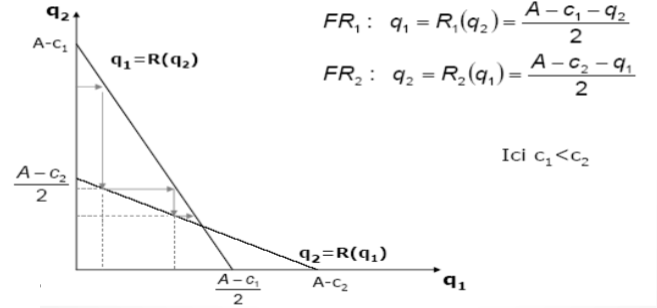
\includegraphics[scale=0.8]{Pics/Duopole_cournot.png}
\newpage
\subsection{Duopole de Bertrand}
La valeur stratégique de l'entreprise est le prix. La fonction de demande du marché $D$ s'exprime en fonction du prix $p$ fixé par les deux entreprises.
Lorsque les prix fixés sont différents, on note $\forall i \in \{1,2\}, D_{i}$ la fonction demande du marché pour l'entreprise $i$. La demande sera adressée à l'entreprise ayant le prix le plus faible.
\[
\left \{
\begin{array}{c}
    D_{1} = D(p_{1}), D(p_{2}) = 0 ;p_{1} < p_{2}\\
    D_{1} = D_{2} = \frac{D(p_{1})}{2} =  \frac{D(p_{2})}{2} ;p_{1} = p_{2}\\
    D_{2} = D(p_{2}), D(p_{1}) = 0 ;p_{2} < p_{1}
\end{array}
\right.
\]
\begin{itemize}
    \item Si $c_{1} = c_{2} = c$, la maximisation du profit $\pi_{i}$ pour les entreprises est : \newline
    \textcolor{White}{.}
    \begin{center}
        \Large{\fbox{$\pi_{i}(q_{i}) = (p_{i} - c)q_{i}$ avec $CT_{i}(q_{i}) = cq_{i}$}}
    \end{center}
    \textcolor{White}{.}
    \item Si $CT{i}(q_{i}) = c_{i}q_{i}$ et $CT{j}(q_{j}) = c_{j}q_{j}$ avec $c_{i} < c_{j}$, la maximisation du profit $\pi_{i}$ de l'entreprise i est : \newline
    \textcolor{White}{.}
    \begin{center}
        \Large{\fbox{$\pi_{i}(q_{i}) = D(c_{j})(c_{j} - c_{i})$}}
    \end{center}
    \textcolor{White}{.}
    \item Le coût moins élevé de l'entreprise 1 permet de s'accaparer la demande. La maximisation du profit pour les deux entreprises mènent à $p_{1} = p_{2} = c$. \textbf{L'équilibre de Bertrand mène au même résultats que la concurrence parfaite : profits nuls pour les entreprises à condition que les deux entreprises agissent de la même manière}
\end{itemize}
\newpage
\subsection{Duopole de Stackelberg}
Dans le cas d'un duopole de Stackelberg, une entreprise est en position dominante, \textbf{leader} et l'autre la suit, elle est \textbf{follower}. L'entreprise \textbf{leader} prend des décisions que l'autre entreprise ne peut contester et \textbf{anticipe ses réactions}. \newline
\begin{itemize}
    \item Maximisation du profit du \textbf{follower} (entreprise 2) : \newline
    \textcolor{White}{.}
    \begin{center}
        \Large{\fbox{$
        max \pi_{2}(q_{1},q_{2}) = p(q_{1},q_{2})q_{2} - c_{2}q_{2}
        $}}
    \end{center}    \textcolor{White}{.}
    \item Conditions de premier ordre : \newline
    \textcolor{White}{.}
    \begin{center}
        \Large{\fbox{$
        \frac{\partial \pi_{2}(q_{1},q_{2})}{\partial q_{2}} = 0
        $}}
    \end{center}
    \textcolor{White}{.}
    \item Fonction de réaction (identique à celle du duopole de Cournot) : \newline
    \textcolor{White}{.}
    \begin{center}
        \Large{\fbox{$
        q_{2} = R_{2}(q_{1}) = \frac{A - c_{2} - q_{1}}{2}
        $}}
    \end{center}
    \textcolor{White}{.}
    \item L'entreprise 1 connaît la façon de réagir de l'entreprise 2 : \newline
    \textcolor{White}{.}
    \begin{center}
        \Large{\fbox{$
        max \pi_{1}(q_{1},q_{2}) = p(q_{1},q_{2})q_{1} - c_{1}q_{1}
        $}}
    \end{center}
    Sachant que :
    \begin{center}
        \Large{\fbox{$
        q_{2} = R_{2}(q_{1}) = \frac{A - c_{2} - q_{1}}{2}
        $}}
    \end{center}
    \textcolor{White}{.}
    \item Conditions de premier ordre : \newline
    \textcolor{White}{.}
    \begin{center}
        \Large{\fbox{$
        \frac{\partial \pi_{1}(q_{1},q_{2})}{\partial q_{1}} = 0
        $}}
    \end{center}
\end{itemize}
\newpage
On a alors : 
\begin{center}
    \Large{\fbox{$
    q_{1} = \frac{A - 2c_{1} + c_{2}}{2}
    $}}
    \Large{\fbox{$
    q_{2} = \frac{A - 2c_{1} + c_{2}}{4}
    $}}
\end{center} 
Les quantités produites par l'entreprise 2 étant anticipées par l'entreprise 1, \textbf{l'entreprise leader peut produire plus qu'en situation de duopole de Cournot tandis que l'entreprise 2 produit moins, ce qui souligne l'avantage qu'à l'entreprise 1 sur l'entreprise 2.}
\newpage
\subsection{Entente collusive ou cartel}
Les entreprises peuvent envisager des ententes entre elles : elles forment un cartel qui se comporte comme un monopole avec plusieurs établissements et prix. \textbf{\Large{Le but est de maximiser la somme des profits des entreprises}}\newline
Ce type d'entente \textbf{n'est pas stable} : il y a généralement des non-respects de ces ententes.
\begin{center}
    \Large{\fbox{$max \pi = \pi_{1} + \pi_{2} = p(q_{1},q_{2})(q_{1} + q_{2}) - C_{1}(q_{1}) - C_{2}(q_{2})$}}
\end{center}
Conditions de premier ordre :
\begin{center}
   \fbox{\Large{$\forall i \in \{1,2\},$} \huge{$\frac{\partial \pi}{\partial q_{i}} = 0$}}
\end{center}
A l'équilibre : \Large{{$C_{m_{1}} = C_{m_{2}}$} \newline

Matrice des décisions :
\begin{center}
    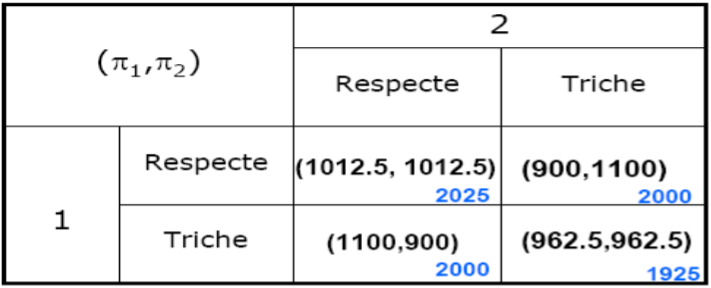
\includegraphics[scale=0.9]{Pics/Matrice_des_decisions.png}
\end{center}
